\documentclass[10pt]{beamer}

\usetheme[progressbar=frametitle]{metropolis}
\usepackage{appendixnumberbeamer}

\usepackage{booktabs}
\usepackage[scale=2]{ccicons}

\usepackage{pgfplots}
\usepgfplotslibrary{dateplot}

\usepackage{xspace}
\newcommand{\themename}{\textbf{\textsc{metropolis}}\xspace}

\usepackage{array}
\usepackage{adjustbox}
\usepackage{ragged2e}

% Enables row styling (ex. make whole row bold texted)
\newcolumntype{`}{>{\global\let\currentrowstyle\relax}}
\newcolumntype{^}{>{\currentrowstyle}}
\newcommand{\rowstyle}[1]
{\gdef\currentrowstyle{#1}%
  #1\ignorespaces
}

\title{Question-Comment Similarity in Community Q\&A forums}
\subtitle{Master's Thesis Presentation}
% \date{\today}
\date{}
\author{Sandesh C \newline 12CS30041}
\institute{Under the supervision of: \newline \newline Prof. Pawan Goyal \newline Department of Computer Science and Engineering \newline Indian Institute of Technology -- Kharagpur}
% \titlegraphic{\hfill
\includegraphics[height=1.5cm]{logo.pdf}}

\begin{document}

\maketitle

\begin{frame}{Table of contents}
  \setbeamertemplate{section in toc}[sections numbered]
  \tableofcontents[hideallsubsections]
\end{frame}

\section{Introduction}

\begin{frame}[fragile]{Motivation}
	\begin{itemize}
	% CQA forums such as Stack Overflow\footnote{https://stackoverflow.com/} and Qatar Living\footnote{http://www.qatarliving.com/}, have huge popularity online
	\item Community Q\&A forums are seldom moderated and quite open
	% thus they typically have little restrictions, if any, on who can post and who can answer a question
	% On the positive side, this means that one can freely ask any question and can then expect some good, honest comments
	% On the negative side, it takes effort to go through all possible comments and to make sense of them
	\item Need to automate the process of finding good/relevant comments to questions
	\item Ranking the comments according to relevance to the corresponding question
	\end{itemize}
	
	This problem is also referred to as \textbf{Answer Reranking}.
\end{frame}

\section{SemEval '16 Task 3 (Subtask A)}

\begin{frame}{Semantic Evaluation Tasks}
	\begin{itemize}
	\item Ongoing series of evaluations of computational semantic analysis systems\footnote{http://alt.qcri.org/semeval2016/}
	\item \textbf{Task 3} deals with semantic comparison for words and text in Community Question \& Answering (CQA) domain
	\end{itemize}
	
	\justify
	In essence, the main CQA task can be defined as follows: \\
	\textit{“Given (i) a new question and (ii) a large collection of question-comment threads created by a user community, rank the comments that are most useful for answering the new question”}.
\end{frame}

\begin{frame}{Task 3 -- Subtask A}
In our work we limit ourselves to finding Question-Comment similarity, which comes under the purview of \textit{Subtask A} of \textit{SemEval '16 Task 3}.

\textbf{Subtask A} \textit{Given a question from a question-comment thread, rank the comments as per their relevance (similarity) with respect to the question}.
\end{frame}

\begin{frame}{Exploring the Dataset}
	\setcounter{table}{0}
	\begin{table}[!htbp]
	\centering
	\begin{adjustbox}{max width=\textwidth,center}
	\begin{tabular}{`l^r^r^r^r^r^r}
	\rowstyle{\bfseries}
	Category 			&	Train 		&	Train		&	Train+Dev+Test		&	Dev		&	Test		&	Total	\\
	\rowstyle{\bfseries}
						&	(Part-I)		&	(Part-II)	&	(from SemEval 2015)	&			&			&			\\
	\\\hline\\
	\rowstyle{\bfseries}
	Questions			&	1,411		&	379			&	2,480+291+319		&	244		&	327		&	5,451	\\\\
	\rowstyle{\bfseries}
	Comments				&	14,110		&	3,790		&	14,893+1,529+1,876	&	2,440	&	3,270	&	41,908	\\
	\rowstyle{\itshape}
	-Good				&	5,287		&	1,364		&	7,418+813+946		&	818		&	1,329	&	17,975	\\
	\rowstyle{\itshape}
	-Bad					&	6,362		&	1,777		&	5,971+544+774		&	1,209	&	1,485	&	18,122	\\
	\rowstyle{\itshape}
	-Potentially			&	2,461		&	649			&	1,504+172+156		&	413		&	456		&	5,811	\\
	\hline
	\end{tabular}
	\end{adjustbox}
	\caption{English CQA-QL corpus from SemEval-2017 Task 3 (Subtask A)}
	\label{table:data}
	\end{table}
\end{frame}

\section{Gimplse at relevant Literature}

\begin{frame}{Literature Review}
	Recent works which attempt to solve the problem of answer re-ranking:
	\begin{itemize}
	\item \cite{lin2015icrc} treated the answer selection task as a sequence labeling problem and proposed recurrent convolutional neural networks to recognize good comments
	\item \cite{zhou2015answer} included long-short term memory (LSTM) units in their convolutional neural network to learn the classification sequence for the thread
	% \item \cite{barron2015thread} exploited the dependencies between the thread comments to tackle the same task by designing features that look globally at the thread
	\end{itemize}
\end{frame}

\begin{frame}{SemEval '16 Task 3 -- Subtask A}
\begin{itemize}
\item Notably, at SemEval '16 Task 3 -- Subtask A provided a great set of Tree Kernel based approaches, that proved to give best results, out performing various LSTM based approaches \item Although the reason for this could be for the lack of substantial data for an LSTM to be trained over
\end{itemize}
\end{frame}

%\begin{frame}{Tree Kernel based approaches}
%\justify
%\cite{filice2016kelp}, being the best submission at SemEval '16 Task 3 -- Subtask A, gave an SVM learning algorithm that operates on a linear combination of kernel functions, each one applied over a specific representation of the targeted examples:
%\begin{itemize}
%\item feature vectors containing linguistic similarities between Q \& A texts
%\item shallow syntactic trees that encode the lexical and morpho-syntactic information shared between these text pairs
%\item feature vectors capturing task-specific information.
%\end{itemize}
%\end{frame}

\begin{frame}{Approaches based on feature engineering}
\justify
\cite{mihaylov2016semanticz} on the other hand constructs various semantic and metadata features and trains an SVM to the solve the classification problem of comment relevance.

This idea of using various helpful features from metadata and constructing scores for the similarity between the semantics of question and comment text has been adopted in our approach as well owing to it's simplicity.
\end{frame}

\section{Approach}

\begin{frame}{Neural Approach}
	\begin{itemize}
	\item A neural approach to open-domain non-factoid Question-Answering introduced by \cite{bogdanova2016we}
	\item Question-comment pairs represented as concatenated distributed representation vectors
	\item Multilayer Perceptors to compute similarity scores
	\end{itemize}

\justify
Despite its simplicity, their work achieved \textbf{state-of-the-art} performance on the Yahoo! Answers dataset of manner or How questions \cite{jansen2014discourse}.

This improved performance was attributed to the use of \textbf{paragraph vector} representations instead of averaging over word vectors.
\end{frame}
	
	% We used a simple feedforward neural network, i.e. a multilayered perceptron, to predict the best answer, similar to the apporach in \cite{bogdanova2016we}. As shown in \autoref{fig:ann-arch}, the first layer of network takes the vector representation for a question-comment pair \textit{(q, c)} as input, which is a concatenation of the distributed representations \textit{q} and \textit{c}, the question and the comment text respectively. Each representation is a real-valued vector of a fixed dimensionality \textit{d}, which is a parameter to be tuned. The input layer is concatenated with another \textit{d} dimensional vector, namely the centroidal comment, which is centroid of the distributed representation of all comments to the question q (\autoref{subsection:centroidal-comment}). This is further concatenated with another set of features, that capture syntactic and metadata information, generated from the pair (q, c) as described in \autoref{subsection:feature-set}. The latter two enhancements is the reason our approach shall improve upon the performance achieved by \cite{bogdanova2016we}.

\begin{frame}{Proposed Architecture}
	\begin{figure}[t!]
	  \centering
	  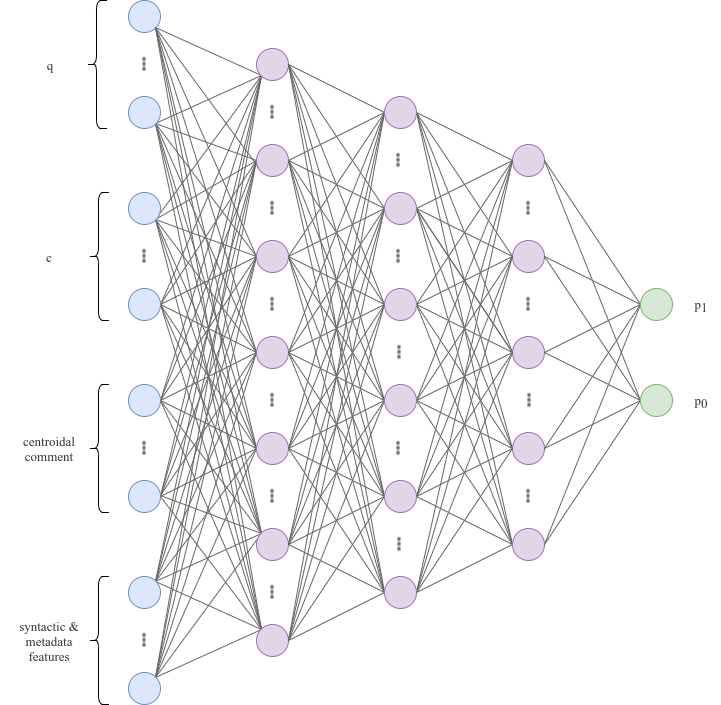
\includegraphics[keepaspectratio, scale=0.275]{./Pictures/ann-arch.png}
	  \caption{Architecture of proposed Feedforward Neural Network}
	  \label{fig:ann-arch}
	\end{figure}
\end{frame}

\begin{frame}{Centoridal Comment}
\[ avg\_com_q = \frac{\sum\limits_{c \in q} c}{||\sum\limits_{c \in q} c||} \tag{1} \label{equation:1} \]

\begin{itemize}
\item Using the information in other comment texts
\item Intended to capture the inter-dependency at thread level
\item Results in accurate relative relevance scores as output probability is the inverse rank for comment texts
\end{itemize}
\end{frame}

\begin{frame}{Syntactic \& Semantic Features I}

Cosine Similarity
\[ sim(u, v) = 1 - \frac{u.v}{||u||.||v||} \tag{2} \label{equation:2} \]

Centroid Vector
\[ centroid(w_{1...n}) = \frac{\sum\limits_{i=1}^{n} w_i}{n} \tag{3} \label{equation:3} \]

\end{frame}

%\begin{frame}{Syntactic \& Semantic Features II}
%\justify
%\textbf{Question to Answer similarity.} We assume that relevant answer should have a centroid vector that is close to that for the question.
%
%\textbf{Maximized similarity.} Average similarity of the top N words (words from comment text most similar to question text). We took the top 1, 2, 3, 4 and 5 words similarities as features.
%
%The assumption here is that if the average similarity for the top N most similar words is high, then the comment might be relevant.
%
%\textbf{Aligned similarity.} For each word in the question text, we chose the most similar word from the comment text and we took the average of all best word pair similarities as suggested in \cite{tran2015jaist}.
%\end{frame}

\begin{frame}{Syntactic \& Semantic Features II}
\justify
\textbf{Part of speech (POS) based word vector similarities.} We performed part of speech tagging using the Stanford tagger \cite{toutanova2003feature}, and we took similarities between centroid vectors of words with a specific tag from the comment text and the centroid vector of the words with a specific tag from the question text.

The assumption is that some parts of speech between the question and the comment might be closer than other parts of speech.

\textbf{Word clusters (WC) similarity.} We clustered the word vectors from the Word2Vec vocabulary in 1,000 clusters using K-Means clustering. We then calculated the cluster similarity between the question text word clusters and the answer text word clusters.
\end{frame}

\begin{frame}{Syntactic \& Semantic Features III}
\justify
\textbf{LDA topic similarity.} 
\begin{itemize}
\item Topic clustering using Latent Dirichlet Allocation (LDA) as implemented in the gensim \cite{rehurek2010software} toolkit on Train1 + Train2 + Dev questions and comments. 
\item We built topic models with 100 topics. 
\item For words in the question text and comment text, we built a bag-of-topics, and calculated similarity. 
\end{itemize}
The assumption here is that if the question and the comment share similar topics, they are more likely to be relevant to each other.

\textbf{Paragraph Vector similarities.} The similarity between the distributed vector representations of question text (\textit{q}), answer text (\textit{a}) and the centroidal comment ($avg\_com_q$), taken two at a time are also included.
\end{frame}

\begin{frame}{Metadata Features I}
\justify
\textbf{Answer contains a question mark.} If the comment has an question mark, it may be another question, which might indicate a bad answer.

\textbf{Answer length.} Assumption here is that longer answers could bring useful details.

\textbf{Question length.} If the question is longer, it may be more clear, which may help users give a more relevant answer.

\textbf{Question to comment length.} If the question is long and the answer is short, it may be less relevant.
\end{frame}

\begin{frame}{Metadata Features II}
\justify
%\textbf{Answer's author and the corresponding question's author are same.} If the answer is posted by the same user who posted the question and it is relevant, why has he/she asked the question in the first place?
%
%\textbf{Answer rank in the thread.} Earlier answers could be posted by users who visit the forum more often, and they may have read more similar questions and answers. Moreover, discussion in the forum tends to diverge from the question over time.

\textbf{Question category.} We took the category of the question as a sparse binary feature vector (a feature with a value of 1 appears if question is in the category). The assumption here is that the question-comment relevance might depend on the category of the question.

\textbf{Time difference between Question and Comment posting.} Immediate comments could reflect incomplete answers to longer questions, while comments posted after substantial time might reflect well-thought answers.
\end{frame}

%\begin{frame}{Metadata Features III}
%\justify
%\textbf{Comments by the same User.} The number of comments by the author of a given comment to the same question and the order of the comments (first, second, ...) is also included as a feature. If the author produced an incomplete answer in the first attempt, he/she might be obliged to produce another comment subsequently.
%
%\textbf{Time difference between Question and Comment posting.} Immediate comments could reflect incomplete answers to longer questions, while comments posted after substantial time might reflect well-thought answers.
%\end{frame}

\section{Paragraph Vector Representation}

\begin{frame}{Summary}
\begin{itemize}
\item Paragraph Vector is an unsupervised framework that learns continuous distributed vector representations for variable-length pieces of texts.
\item We experimentally evaluate the Paragraph Vector (PV) model proposed by \cite{le2014distributed}.
\item PV is an extension of the widely used continuous bag-of-words (CBOW) and skip-gram word embedding models, known as word2vec.
\end{itemize}
\end{frame}

\begin{frame}{Distributed Memory (DM) framework}
	\begin{figure}[t!]
	  \centering
	  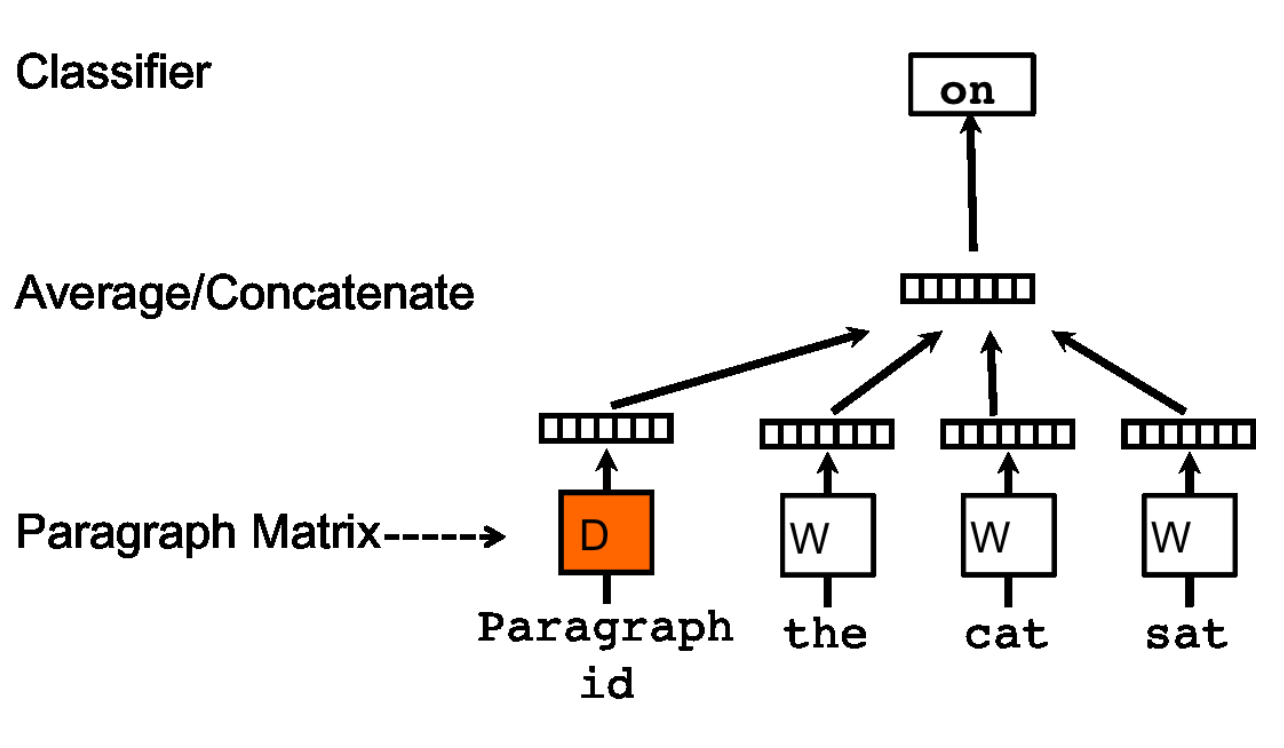
\includegraphics[keepaspectratio, width=0.8\textwidth]{./Pictures/pv-dm.png}
	  \label{fig:pv-dm}
	\end{figure}
	
	\begin{itemize}
	\item Concatenation or average of word vectors with a context of few words is used to predict the next word.
	\item PV represents the missing information from the current context and can act as a memory of the topic of the paragraph.	
	\end{itemize}
\end{frame}

\begin{frame}{Distributed Bag of Words (DBOW) framework}
	\begin{figure}[t!]
	  \centering
	  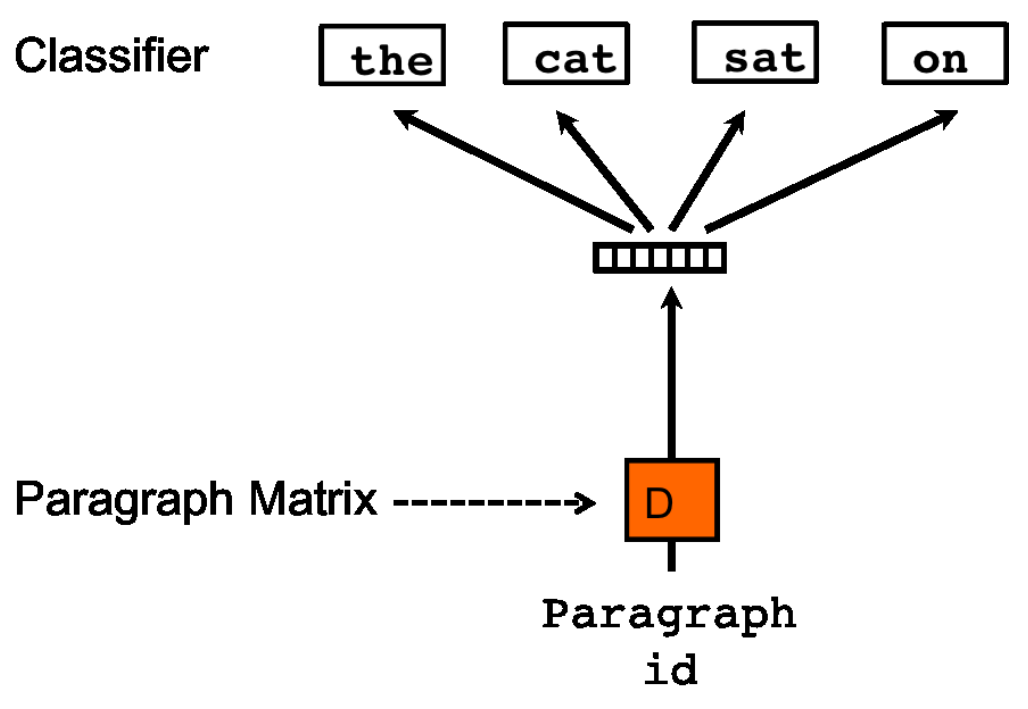
\includegraphics[keepaspectratio, width=0.8\textwidth]{./Pictures/pv-dbow.png}
	  \label{fig:pv-dbow}
	\end{figure}
	The paragraph vector is trained to predict the words in a small window.
\end{frame}

\begin{frame}{Training Paragraph Vectors}
	
\begin{itemize}
\item We use the \textit{gensim}\footnote{https://radimrehurek.com/gensim/models/doc2vec.html} implementation of DM and DBOW paragraph vector models
\item Data for training the unsupervised \textit{doc2vec} model is a large unannotated dataset from Qatar Living forums ($\sim$2.3M samples)
\item Each piece of text was converted to lowercase, tokenized (by numerics and special characters) and cleaned of stop words
\end{itemize}

\end{frame}

\begin{frame}{Framework of PVs -- DBOW vs DM}
	\begin{table}[!htbp]
	\centering
	\begin{adjustbox}{max width=\textwidth,center}
	\begin{tabular}{`c^c^c^c^c^c^c^c}
	\rowstyle{\bfseries}
	Category 			&	Window 	&	Epochs	&	Normalized	&	Norm. Sq. Error	&	Ratio\\
	\rowstyle{\bfseries}
						&	Size		&			&	Sq. Error (A)	&	(Random)	(B)		&	(B/A)\\
	\\\hline\\
	PV-DBOW & 10 & 5 & 0.14 & 0.80 & 5.89 \\
	PV-DBOW & 10 & 10 & 0.14 & 0.83 & 5.84 \\
	PV-DM & 10 & 5 & 0.21 & 0.99 & 4.67 \\
	PV-DM & 15 & 10 & 0.22 & 0.98 & 4.47 \\
	\hline
	\end{tabular}
	\end{adjustbox}
	\caption{Training document vector representations -- Best results}
	\label{table:pv-train-best}
	\end{table}
	
	\begin{itemize}
	\item \textbf{Window size} is the maximum distance between the predicted word and context words used for prediction within a document
	\item \textbf{Epochs} is the number of iterations for which the \textit{doc2vec} model is trained over dataset
	\item Note that dimensions of the PVs in these experiments are 100
	\end{itemize}
\end{frame}

\begin{frame}{Dimension of PVs -- 100 vs 200 }
\begin{table}[!htbp]
\centering
\begin{adjustbox}{max width=\textwidth,center}
\begin{tabular}{`c^c^c^c^c^c^c^c}
\rowstyle{\bfseries}
Dimension 			&	Window 	&	Epochs	&	Normalized	&	Norm. Sq. Error	&	Ratio\\
\rowstyle{\bfseries}
					&	Size		&			&	Sq. Error (A)	&	(Random)	(B)		&	(B/A)\\
\\\hline\\
100 & 10 & 5 & 0.14 & 0.80 & 5.89 \\
100 & 10 & 10 & 0.14 & 0.83 & 5.84 \\
200 & 10 & 10 & 0.15 & 0.84 & 5.65 \\
200 & 10 & 5 & 0.15 & 0.82 & 5.47 \\
\hline
\end{tabular}
\end{adjustbox}
\caption{Training PV-DBOW vectors of sizes 100 \& 200 -- Best results}
\label{table:pv-dimen-best}
\end{table}
\end{frame}

\section{Experimental Setup}

\begin{frame}{Experimental Setup}
\begin{itemize}
\item For the implementation of the feedforward neural network we used the popular python library \textit{scikit-learn\footnote{http://scikit-learn.org/stable/index.html}}'s \textit{MLPClassifier}\footnote{http://scikit-learn.org/stable/modules/generated/sklearn.neural\_network.MLPClassifier.html}
\item Training data comprises of 38,638 comments over 5,124 questions
\item The neural net input is a tuple of the form $(q, c, avg\_ans_q, ft_{(q,c)})$
\item Nets were trained with parameters being the solvers, activation functions and hidden layer configurations
\end{itemize}
\end{frame}

\begin{frame}{Evaluation Metrics}
\justify
\textbf{SemEval Task 3} has as an official evaluation measure used to rank the participating systems, the metric of Mean Average Precision (\textit{MAP}), calculated for the ten comments a participating system has ranked highest. 

Further metrics such as Mean Reciprocal Rank (\textit{MRR}) and Average Recall (\textit{AvgRec}) for top-10 results; Precision (\textit{P}), Recall (\textit{R}), \textit{F\textsubscript{1}} (with respect to the Good/Relevant class) and Accuracy (\textit{Acc}) are also reported.
\end{frame}

\section{Results}

\begin{frame}{Preliminary experiments with $(q, c)$ inputs}
	\begin{table}[!htbp]
	\centering
	\begin{adjustbox}{max width=\textwidth,center}
	\begin{tabular}{`c^c^c^c^c^c^c^c^c^c}
	\rowstyle{\bfseries}
	Category & Solver & Activation & MAP & AvgRec & MRR & P & R & F\textsubscript{1} & Acc \\
	\\\hline\\
	PV-DBOW & Adam & logistic & \textbf{70.49} & 82.92 & 77.62 & 66.01 & 55.08 & 60.05 & 70.21 \\
	PV-DBOW & SGD & relu & 70.19 & 82.51 & 77.16 & 63.27 & 59.37 & 61.26 & 69.48 \\
	PV-DBOW & SGD & logistic & 70.18 & 82.42 & 77.32 & 64.12 & 58.77 & 61.33 & 69.88 \\
	PV-DBOW & SGD & tanh & 70.09 & 82.45 & 76.62 & 63.39 & 59.14 & 61.19 & 69.51 \\
	PV-DBOW & Adam & relu & 69.93 & 81.06 & 76.94 & 59.98 & 57.41 & 58.67 & 67.13 \\
	PV-DBOW & Adam & tanh & 69.80 & 82.31 & 76.35 & 63.86 & 55.46 & 59.36 & 69.14 \\
	PV-DM & SGD & relu & 65.78 & 78.55 & 74.58 & 57.93 & 53.57 & 55.67 & 65.32 \\
	\hline
	\end{tabular}
	\end{adjustbox}
	\caption{Preliminary experiments using only $(q, c)$ inputs -- Best results}
	\label{table:ann-stage-1-best}
	\end{table}
\end{frame}

\begin{frame}{Improvement with inclusion of Centroidal comment}
	\begin{table}[!htbp]
	\centering
	\begin{adjustbox}{max width=\textwidth,center}
	\begin{tabular}{`c^c^c^c^c^c^c^c^c^c}
	\rowstyle{\bfseries}
	Category & Solver & Activation & MAP & AvgRec & MRR & P & R & F\textsubscript{1} & Acc \\
	\\\hline\\
	PV-DBOW & SGD & relu & \textbf{73.06} & 84.16 & 79.61 & 66.07 & 57.86 & 61.69 & 70.8 \\
	PV-DBOW & SGD & tanh & 71.88 & 83.43 & 79.11 & 66.84 & 56.58 & 61.29 & 70.95 \\
	PV-DBOW & SGD & logistic & 71.79 & 83.46 & 79.13 & 66.52 & 55.3 & 60.39 & 70.52 \\
	PV-DBOW & Adam & logistic & 71.77 & 83.42 & 78.96 & 66.35 & 57.26 & 61.47 & 70.83 \\
	PV-DBOW & Adam & tanh & 71.69 & 83.39 & 78.64 & 65.5 & 57.71 & 61.36 & 70.46 \\
	PV-DBOW & Adam & relu & 71.61 & 82.63 & 79.45 & 62.98 & 60.05 & 61.48 & 69.42 \\
	\hline
	\end{tabular}
	\end{adjustbox}
	\caption{Experiments using $(q, c, avg\_com_q)$ inputs -- Best results}
	\label{table:ann-stage-2-best}
	\end{table}
\end{frame}

\begin{frame}{Further improvement with Syntactic and Metadata Features}
	\begin{table}[!htbp]
	\centering
	\begin{adjustbox}{max width=\textwidth,center}
	\begin{tabular}{`c^c^c^c^c^c^c^c^c^c}
	\rowstyle{\bfseries}
	Category & Solver & Activation & MAP & AvgRec & MRR & P & R & F\textsubscript{1} & Acc \\
	\\\hline\\
	PV-DBOW & SGD & tanh & \textbf{77.74} & 88.2 & 85.58 & 70.81 & 63.51 & 66.96 & 74.53 \\
	PV-DBOW & SGD & relu & 77.43 & 87.96 & 84.81 & 70.57 & 62.6 & 66.35 & 74.19 \\
	PV-DBOW & SGD & logistic & 77.26 & 87.87 & 85.51 & 71.49 & 63.58 & 67.3 & 74.89 \\
	\hline
	\end{tabular}
	\end{adjustbox}
	\caption{Experiments using $(q, c, avg\_com_q, ft_{(q,c)})$ inputs -- Best results}
	\label{table:ann-stage-3-best}
	\end{table}
\end{frame}

\begin{frame}{Analysis with $(q, c, ft_{(q,c)})$ inputs}
	\begin{table}[!htbp]
	\centering
	\begin{adjustbox}{max width=\textwidth,center}
	\begin{tabular}{`c^c^c^c^c^c^c^c^c^c}
	\rowstyle{\bfseries}
	Category & Solver & Activation & MAP & AvgRec & MRR & P & R & F\textsubscript{1} & Acc \\
	\\\hline\\
	PV-DBOW & SGD & logistic & \textbf{77.22} & 87.44 & 84.67 & 69.62 & 62.75 & 66.01 & 73.73 \\
	PV-DBOW & SGD & tanh & 77.14 & 87.44 & 84.65 & 69.31 & 63.21 & 66.12 & 73.67 \\
	PV-DBOW & SGD & relu & 77.03 & 87.39 & 84.8 & 70.32 & 62.75 & 66.32 & 74.10 \\
	\hline
	\end{tabular}
	\end{adjustbox}
	\caption{Experiments using $(q, c, ft_{(q,c)})$ inputs -- Best results}
	\label{table:ann-stage-2half-best}
	\end{table}
\end{frame}

\begin{frame}{Analysis with only $(ft_{(q,c)})$ inputs}
	\begin{table}[!htbp]
	\centering
	\begin{adjustbox}{max width=\textwidth,center}
	\begin{tabular}{`c^c^c^c^c^c^c^c^c^c}
	\rowstyle{\bfseries}
	Category & Solver & Activation & MAP & AvgRec & MRR & P & R & F\textsubscript{1} & Acc \\
	\\\hline\\
	PV-DBOW & SGD & tanh & \textbf{75.11} & 86.63 & 81.78 & 69.93 & 59.14 & 64.08 & 73.06 \\
	PV-DBOW & SGD & relu & 74.84 & 86.25 & 81.61 & 70.09 & 59.59 & 64.42 & 73.24 \\
	PV-DBOW & SGD & logistic & 74.33 & 85.98 & 81.35 & 68.96 & 59.67 & 63.98 & 72.69 \\
	\hline
	\end{tabular}
	\end{adjustbox}
	\caption{Experiments using $(ft_{(q,c)})$ inputs -- Best results}
	\label{table:ann-stage-only-ft-best}
	\end{table}
\end{frame}

\section{Conclusion}

\begin{frame}{Summary}
	\begin{table}[!htbp]
	\centering
	\begin{adjustbox}{max width=\textwidth,center}
	\begin{tabular}{`c^c^c^c^c^c^c^c^c^c}
	\rowstyle{\bfseries}
	Features & MAP & AvgRec & MRR & P & R & F\textsubscript{1} & Acc \\
	\\\hline\\
	$(q, c)$ & \textbf{70.49} & 82.92 & 77.62 & 66.01 & 55.08 & 60.05 & 70.21 \\\\
	$(q, c, avg\_com_q)$ & \textbf{73.06} & 84.16 & 79.61 & 66.07 & 57.86 & 61.69 & 70.8 \\\\
	$(ft_{(q,c)})$ & \textbf{75.11} & 86.63 & 81.78 & 69.93 & 59.14 & 64.08 & 73.06 \\\\
	$(q, c, ft_{(q,c)})$ & \textbf{77.22} & 87.44 & 84.67 & 69.62 & 62.75 & 66.01 & 73.73 \\\\
	$(q, c, avg\_com_q, ft_{(q,c)})$ & \textbf{77.74} & 88.2 & 85.58 & 70.81 & 63.51 & 66.96 & 74.53 \\\\
	\hline
	\end{tabular}
	\end{adjustbox}
	\caption{Best results corresponding to each of the feature sets}
	\label{table:conclusion}
	\end{table}
\end{frame}

\begin{frame}{Comparing with best submissions at SemEval-2016}
	\begin{table}[!htbp]
	\centering
	\begin{adjustbox}{max width=\textwidth,center}
	\begin{tabular}{`l^c^c^c^c^c^c^c^c^c}
	\rowstyle{\bfseries}
	Submission & MAP & AvgRec & MRR & P & R & F\textsubscript{1} & Acc \\
	\hline
	Kelp-primary \cite{filice2016kelp} & 79.19 & 88.82 & 86.42 & 76.96 & 55.30 & 64.36 & 75.11 \\
	ConvKN-contrastive1 \cite{joty2016convkn} & 78.71 & 88.98 & 86.15 & 77.78 & 53.72 & 63.55 & 74.95 \\
	\rowstyle{\bfseries}
	Our Approach & 77.74 & 88.2 & 85.58 & 70.81 & 63.51 & 66.96 & 74.53 \\
	SUper\_team-contrastive1 \cite{mihaylova2016super} & 77.68 & 88.06 & 84.76 & 75.59 & 55.00 & 63.68 & 74.50 \\
	ConvKN-primary \cite{joty2016convkn} & 77.66 & 88.05 & 84.93 & 75.56 & 58.84 & 66.16 & 75.54 \\
	SemanticZ-primary \cite{mihaylov2016semanticz} & 77.58 & 88.14 & 85.21 & 74.13 & 53.05 & 61.84 & 73.39 \\
	\hline
	Baseline (chronological) & 59.53 & 72.60 & 67.83 & — & — & — & — \\
	Baseline (random) & 52.80 & 66.52 & 58.71 & 40.56 & 74.57 & 52.55 & 45.26 \\
	Baseline (all ‘true’) & — & — & — & 40.64 & 100.00 & 57.80 & 40.64 \\
	Baseline (all ‘false’) & — & — & — & — & — & — & 59.36 \\
	\hline
	\end{tabular}
	\end{adjustbox}
	\caption{Best submissions and Baselines for SemEval '16 Task 3 -- Subtask A}
	\label{table:semeval-best}
	\end{table}
\end{frame}

\begin{frame}{Discussions}
\begin{itemize}
\item Our best result has a higher recall value compared to the best submissions at the event
\item Infact our method produces the best $F_{1}$ score out of all the submissions at the event
\end{itemize}
\end{frame}

\begin{frame}{Future Work}
\begin{itemize}
\item With each inclusion of a new set of features there has been an improvement in the MAP score.
\item Further inclusion of features related to syntactic similarity amongst the question, comment text and the centroidal comment, hence is highly likely to be fruitful.
\item Using syntax trees of these text pieces to extract more syntactic \& semantic similarities is a possible start.
\end{itemize}
\end{frame}

\begin{frame}[standout]
  Questions
\end{frame}

\begin{frame}[allowframebreaks]{References}

  \bibliographystyle{apalike}
  \bibliography{main}

\end{frame}

\end{document}